%%%%%%%%%%%%%%%%%%%%%%%%%%%%%%%%%%%%%%%%%%%%%%%%%%%%%%%%%%%%%%%%%
% 卒論,修論用のテンプレート
%%%%%%%%%%%%%%%%%%%%%%%%%%%%%%%%%%%%%%%%%%%%%%%%%%%%%%%%%%%%%%%%%

\documentclass[12pt]{sonota/aislab}

% colorパッケージをgraphicxの前に読み込まないとトラブルになるようである.
% listingsの中でcolorを使用
\usepackage[usenames]{color}
% 図の挿入にgraphicxパッケージを使用.
% dvipdfmxを使用してpdfを作成することを前提とする.
\usepackage[dvipdfmx]{graphicx}
% urlの表記
\usepackage{url}
% \screen などのコマンドを使えるようにする.
\usepackage{ascmac}
% 書体の変更を許すtt環境
\usepackage{alltt}
% \begin{comment} 〜 \end{comment}でコメントアウトするためのコマンド
\usepackage{comment}

\usepackage{url}

%%%%%%%%%%%%%%%%%%%%%%%%%%%%%%%%%%%%
% 李研テンプレートを作成するにあたって追加したパッケージ
% 参考文献を参照する際の\citeの挙動
\usepackage{sonota/styles/cite}
% 図を横に並べる際に使用
\usepackage{sonota/styles/subfigure}
%%%%%%%%%%%%%%%%%%%%%%%%%%%%%%%%%%%%

% 図はfigsのサブディレクトリに集めることにする.
\graphicspath{{./figs/}}

%%%%%%%%%%%%%%%%%%%%%%%%%%%%%%%%%%%%%%%%%%%%%%%%%%%%%%%%%%%%%%%%%
% ページのレイアウトの指定にgeometryパッケージを使用する
%
% jsbookは10ptでタイプセットし,それを12ptに拡大しているので,ここでの
% papersizeの指定は要注意(a4paperを指定すると結果的に縮小される)
% また,jsbookを使っているためtruemmを使う必要あり
\usepackage{geometry}
% 一行 40文字
\geometry{textwidth=40zw}
% テキスト領域を左右中央に
\geometry{hcentering=true}
% 1ページ35行
\geometry{lines=35}
% footnoteとの間を1行分あける
\geometry{footskip=2\baselineskip}
% PDFへの出力を前提として,綴じ代はプリンタドライバの機能に任せる方針で
% 綴じ代はなしにする
\geometry{bindingoffset=0truemm}

%%%%%%%%%%%%%%%%%%%%%%%%%%%%%%%%%%%%%%%%%%%%%%%%%%%%%%%%%%%%%%%%%
% ヘッダ,フッタにfancyhdrを使う
%
\usepackage{fancyhdr}
\fancyhf{}
\fancyfoot[c]{\thepage}
\renewcommand{\headrulewidth}{0pt}
\renewcommand{\footrulewidth}{0pt}
\pagestyle{fancy}
% jsbook.clsでは,chapterの最初のページのpagestyleを
% plainではなく,plainhead ないし plainfootに設定している.
% そこで,plainheadを再定義する.
\fancypagestyle{plainhead}{%
%\fancypagestyle{plain}{%
\fancyhf{}
\fancyfoot[c]{\thepage}
\renewcommand{\headrulewidth}{0pt}
\renewcommand{\footrulewidth}{0pt}
}

%%%%%%%%%%%%%%%%%%%%%%%%%%%%%%%%%%%%%%%%%%%%%%%%%%%%%%%%%%%%%%%%%
% PDF版でしおりを挿入するためのスタイル hyperref
% dvipdfmxを使ってpdfファイルを作成することを前提とする
\usepackage{atbegshi}
\AtBeginShipoutFirst{\special{pdf:tounicode 90ms-RKSJ-UCS2}}
% MacTeX-2011では90ms-RKSJ-UCS2が含まれていない.
% 代わりにEUC-UCS2を指定してもうまく動くようである
%\AtBeginShipoutFirst{\special{pdf:tounicode EUC-UCS2}}
% paper sizeを変えないようにsetpagesize=falseを指定
% しおりに節番号などをつけるようにする.
\usepackage[setpagesize=false,dvipdfm,%
bookmarks=true,bookmarksnumbered=true]{hyperref}
%bookmarks=true,bookmarksnumbered=true,colorlinks=true]{hyperref}

\newcommand{\fig}[1]{
	Fig. #1
}
\newcommand{\tab}[1]{
	Table #1
}
\newcommand{\eq}[1]{
	式(#1)
}

%%%%%%%%%%%%%%%%%%%%%%%%%%%%%%%%%%%%%%%%%%%%%%%%%%%%%%%%%%%%%%%%%
% 卒業論文用テンプレート
%%%%%%%%%%%%%%%%%%%%%%%%%%%%%%%%%%%%%%%%%%%%%%%%%%%%%%%%%%%%%%%%%
% △ここまでプリアンブル△
% △ここまでプリアンブル△
% △ここまでプリアンブル△
\begin{document}
% ▽ここから本文▽
% ▽ここから本文▽
% ▽ここから本文▽

\pdfbookmark[0]{表紙}{cover}
\begin{titlepage}
\centering
\vspace*{3truecm}
\Huge
% ここに卒論の題目を入れる
Dual ubiquitous Displayによる\\
深層強化学習を用いた\\
行動モデルの構築\\
\vfill
\Large
立命館大学\\
情報理工学研究科\\
博士課程前期課程 情報理工学専攻\\[1zh]
学生証番号 6611190063-0\\[0.5zh]
{\LARGE{三木健汰}}\\[2zh]
2021年2月8日
\end{titlepage}


\let\cleardoublepage\clearpage

% ページ番号はローマ数字で
\frontmatter

\clearpage
\pdfbookmark[0]{概要}{abstract}
\chapter*{概要}
本文書は,卒業論文を作成する際のヒントや注意事項を述べる.また,このファ
イル自体が{\LaTeX}を使用して卒業論文を作成する際のテンプレートになること
も想定している.なお,{\LaTeX}を使用する上での注意事項は付録を参照のこと.

概要は論文全体の概要を書くこと.論文の最初に置かれるが,イントロダクション
ではない.結論まで含めて書く.論文執筆の際には本文を全部書きあげてから,
概要を書いた方が書きやすい.

%% 目次
\clearpage
\pdfbookmark[0]{\contentsname}{toc}
\bgroup

% 章の目次
\tableofcontents
% 図の目次
\clearpage
\pdfbookmark[0]{\listfigurename}{lof}
\listoffigures 
% 表の目次 -- 表がない場合は,表目次そのもの削除すること.
\clearpage
\pdfbookmark[0]{\listtablename}{lot}
\listoftables

\egroup

% 本文スタート(ページ番号は算用数字にする)
\mainmatter

\chapter{緒言}\label{chap:introduction}

\section{研究背景}
近年のコンピュータ技術の進歩に伴いスマートフォンなどの小型情報端末が普及してきており,人々はどこでも様々な情報を取得できるようになってきている.そして,FacebookなどのSNS(Social Networking Service)により,簡単に個人の情報をデジタル化し発信することがでできると共に,情報量は膨大となり,情報の種類は多様化している.そのような情報化社会では,人は適切なときに自らが本当に必要な情報を取得するとこは困難になりつつある.こういった問題から,人が情報を探すのではなく,情報から人へ向けた能動的な情報支援に変化してきている..
GPSやbeaconなどによる位置情報を利用し,場所に応じてそのユーザに適した情報提供が可能となっている.しかし,移動時のスマートフォンの利用(歩きスマホ)は,周辺の人物や障害物への衝突や階段からの転落などの様々な問題があり,その危険性が報告されている\cite{aruki}.また,スマートフォンなどを持っていないユーザへは情報提供が行えない問題点もある.一方,環境設置型の情報提供手段として,駅構内や大型公共施設に設置された自動電子販売機や電子看板などにおいて,カメラを用いて利用者の性別や年齢などの特徴を取得し,その利用者の好みに応じた商品を推薦するシステムもある.しかし,こういった環境接地型の情報提供では,ユーザがその場所まで行く必要があるといった問題がある.
\\ \indent
これに対し,ユーザがスマートフォンなどの端末を持つ必要がなく,また情報提供場所まで行く必要がない情報提示を目指し,移動ロボットを用いた情報提示が行われている\cite{spencr}\cite{UD}.これらのロボットは,これまでの単調な作業を行うだけでなく,空港やショッピングモールといった公共空間において,タッチディスプレイやプロジェクタを搭載した移動ロボットを用いて,人に視覚的な情報の支援を目的として開発されてきたコミュニケーションロボットの一例である.
\section{先行研究}
以上のニーズを踏まえ,立命館大学李研究室では人に対して効果的に情報を提供しコミュニケーションを行うロボットとして,Ubiquitous Display(以後 UD と呼ぶ)の研究・開発を行ってきた\cite{UD1}\cite{UD2}\cite{UD3}\cite{UD4}\cite{UD5}.UD は移動プラットフォームに,パン・チルト回転機構とプロジェクタを搭載した移動型情報投影ロボットである.UD 自らが移動しプロジェクタにより情報を提供することで視覚的情報支援を行うことができる(Fig.\ref{projection}).この投影した視覚情報を用いたインタラクションにより人とコミュニケーションを行うことで,ロボットを用いた新たな情報支援の実現を目指している.これまで,この UD の特徴を活かし室内環境における建物案内システムや投影画像の歪み自動補正,錯視の一つであるアナモルフォーズを用いることで擬似的に立体感を知覚させる裸眼立体投影手法\cite{UD2},知能化空間内のエージェントロボットとして動的環境下において自律的に情報支援を行うための行動モデルの提案\cite{UD5}を行って
きた.

\begin{figure}[t]
\begin{center}
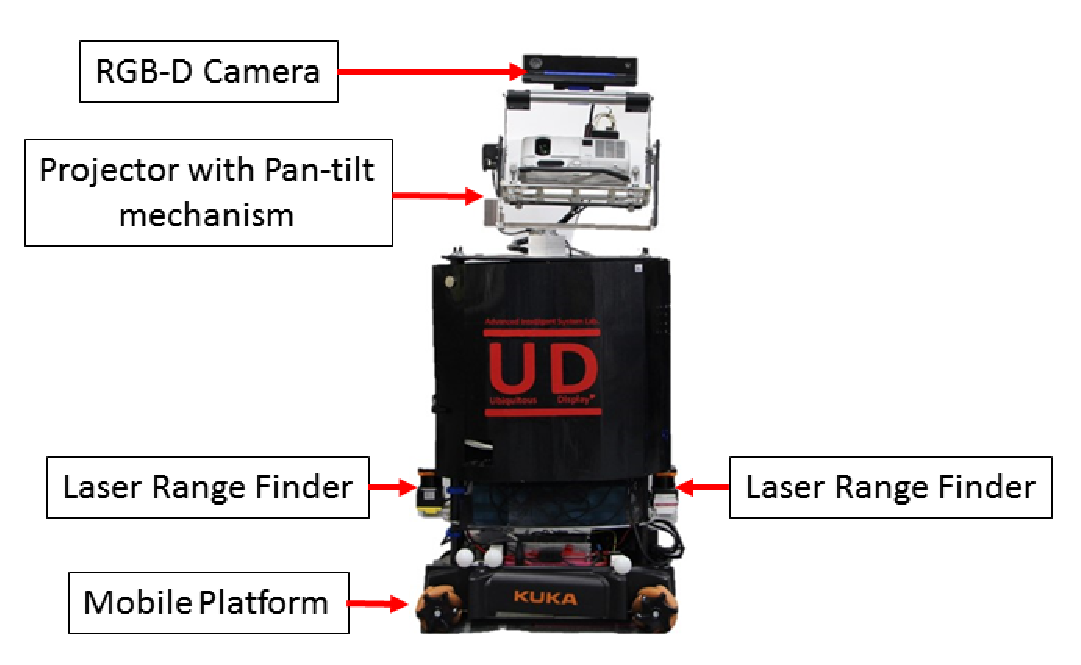
\includegraphics[clip, width=8cm]{figs/ud_with_kinectv2.eps}
\caption{Pictures of Ubiquitous Display}
\label{UD}
\end{center}
\end{figure}

\begin{figure}[t]
\begin{center}
\includegraphics[clip, width=10cm]{figs/demo.JPG}
\caption{Projection information by Ubiquitous Display}
\label{projection}
\end{center}
\end{figure}

\section{関連研究}
本節では,まずはじめに,公共空間において人とコミュニケーションを取り,サービスを提供するロボットの「ふるまい」に関する実験や応用例を紹介する.さらに,人工知能技術の一つである深層強化学習が応用されているロボットの例を紹介する.

\subsection{コミュニケーションロボットの行動制御に関する研究}
近年のロボットの制御技術やセンシング技術の発展や,深層学習の応用により,人とのコミュニケーションや高度な動作制御が可能になった.そして,ロボットは,人の労働力の代替だけでなく,人とインタラクションができ,個人に対するサービスの提供で社会に貢献することが期待されている.しかし,公共空間でロボットが個人にサービス提供を行うためには,まず大勢の不特定多数の中から人をひきつける必要があり,人を意識したロボットの「ふるまい」が求められる.

商業施設などの公共の場所において,案内,情報提供,物資運送などのサービス提供を目的として,様々なコミュニケーションロボットを用いた研究が行われている.Tibelらは,空港内での乗り換えを行う人やグループに対して,大勢の人が行き交う空港の中でも,人を目的地まで案内するロボットを開発している\cite{spencr}.人が動的に動く環境において,安全なナビゲーションを実現するため,FerreらはExtended Social Force Modelを用いた経路計画を提案している\cite{ESTM}.また,これらの人の支援以外の試みとして,Mizuharaらは,警備員の動きを解析し,ショッピングモールで歩きスマホをしている人に忠告する接近方法を提案している\cite{admonishing}.

\subsection{深層強化学習とロボット}
近年,ロボットや自動運転車の制御などに深層強化学習の技術が活発に使われている.
強化学習とは機械学習の一種であり,ある環境のもとに置かれたエージェントが,現在の状態を観測し,行動に対する報酬を得ながら,試行錯誤を通して報酬を最大化するための行動戦略を学習するための枠組みである\cite{RL}.
深層強化学習は,学習主体に深層ニューラルネットワークを用いて学習する技術で,入力値が連続の状態空間におけるQ学習を可能にした\cite{drl}.現在は,深層強化学習を用いてあらゆる目的を達成するための「ロボットの行動の最適化」が行われている\cite{Human_level_dqn}\cite{sarl}.

%%% 編集中 %%%
深層強化学習を用いた移動ロボットの行動制御の一例として,カメラやLidarから取得したセンサ信号を直接ニューラルネットに入力して「センサからモータまで」制御を行うend-to-endなナビゲーションが多く研究されている\cite{ete}\cite{Self}\cite{vtr}.Leiらは,LIDARから取得したデータからロボットの速度を出力させることで,事前地図が不要な自律移動を提案した\cite{vtr}.また,コミュニケーションロボットの行動制御に関しても深層強化学習が使われている.Xuanらは,サービスロボットが動的な環境下で,人間の位置や動きなどの状態や人間のグループ間の相互作用などの社会的ルールを組み込んだナビゲーションフレームワーク\cite{human_navigation}を,DQNで学習させたモデルで安全にサービスロボットが制御可能なことを報告している\cite{human_navigation_dqn}.

\section{研究目的}
これまで,大型公共施設内の人が行き交う通路を想定したUDの情報支援を目的とした行動モデルは開発されている.しかし,Dual Ubiquitous Displayにとって最適な行動モデルの開発は行われていない.そこで本研究では,プロジェクタを2個搭載したDual-Ubiquitous Displayを提案し,深層強化学習を用いてD-UDが最適に情報支援を行うための行動モデルの構築を行う.D-UDが最適な行動モデルの構築が可能になれば,より少ない移動距離で多くの人へ効率的な情報支援を期待できる.本行動モデルの優位性について,シミュレータ実験を通して検証し,その結果について述べる.

\section{論文構成}
本論文の構成を以下に述べる.
第2章では,本研究で使用するロボットについて,ハードウェア構成とソフトウェア構成,そして座標系について述べる.第3章では,本論文で提案するロボットによるプロジェクションマッピングを実現するために提案した手法について述べる.第4章では,提案手法の実験を行い,その結果と考察について述べる.第5章では,本論文のまとめと今後の課題について述べる.


\chapter{Dual-Ubiquitous Display: D-UD}\label{chap:d_ud_mechanism}
本章では,本研究室で研究・開発されてきたUbiquitous Display(以下UD)を拡張し,プロジェクタを2つ搭載したロボットDual-Ubiquitous Display(以下D-UD)の概要について述べる.D-UDが提供できる情報投影手法および設計コンセプトを述べたのち,ハードウェア構成とソフトウェア構成についても詳細に述べる.

\section{D-UDの設計コンセプト}
D-UDはプロジェクタを2台搭載する自律移動型投影ロボットである(Fig.\ref{DUD}).これまで,UDは人が情報端末を所持したり,電子掲示板まで移動したりする必要なく情報を支援することを目標に設計コンセプトを設け開発を行ってきた\cite{UD1}.以下にUDの設計コンセプトの詳細を示す.

\begin{itemize}
\item 実環境全てを網羅する描画領域(ユビキタス表示)
\item 描画情報のシームレスな変化(シームレスな表示)
\item 人の行動・意図に対応するサービス(インタラクティブ表示)
\item Wenbと連携したコンテンツの表示(適応表示)
\end{itemize}

D-UDはこれらのコンセプトを引き継ぐと共に,異なる位置の人に同時に情報投影できる効率的な情報支援を行うため,全方向四輪移動プラットフォームにパン・チルト回転機構を搭載したプロジェクタ2台から構成されている(Fig.\ref{DUD}).さらに,周囲360°パノラマ画像が取得可能なカメラと距離30m,270°の範囲をデータ出力するレーザスキャナ(LRF)を搭載し,D-UDの活動環境を広範囲に認識することで人の見やすい場所に情報投影を行う人間中心の視覚的情報支援が可能である.また,D-UDは2つのプロジェクタから映像を投影することで,異なる位置の2人へ同時に投影することが可能であり,UD2.1よりも多くの人への効率的な情報支援を行う.さらに,両プロジェクタの映像を重ね合わせて1つの映像にすることで,映像の切り替えが少なく人に優しい情報支援の提供が可能である.Fig.\ref{fig:twofig}はその具体例を示している.まず,D-UDが人を認識し接近を行う(Fig.\ref{fig:lefttop}).ユーザの前まで到着が完了すると,ユーザの「このフロアのマップを見せてください」という問いかけに対して,左側のプロジェクタでフロアのマップを投影する(Fig.\ref{fig:leftbottom}).そして,ユーザの「理研究室の場所を教えて下さい」という問に対して,左側のプロジェクタで投影したマップの上に,右側で目的の場所に関連した付加情報を投影する(Fig.\ref{fig:rightbottom}).

\begin{figure}[t]
\begin{center}
\includegraphics[clip, width=10cm]{figs/dud_overview.eps}
\caption{Overview of Dual Ubiquitous Display}
\label{DUD}
\end{center}
\end{figure}

%\section{D-UDが提供する情報投影手法}

\begin{figure}[htbp]

	\begin{center}
	\subfigure[Approaching human]{\includegraphics[width=6cm]{figs/dud_1_white.eps}
	\label{fig:lefttop}}
	%\hspace{10mm}
	\subfigure[Arrived in front of user]{\includegraphics[width=6cm]{figs/dud_2.eps}
	\label{fig:righttop}}
	\subfigure[Projection image by left projector]{\includegraphics[width=6cm]{figs/dud_3.eps}
	\label{fig:leftbottom}}
	%\hspace{10mm}
	\subfigure[Projection image by right projector]{\includegraphics[width=6cm]{figs/dud_4.eps}
	\label{fig:rightbottom}}
	\end{center}
	
	\caption{Projection flow of Dual Ubiquitous Display}
	\label{fig:twofig}
\end{figure}

%\section{D-UDによる人への情報支援}


\section{ハードウェア構成}
D-UDを構成するハードウェアの詳細について述べる.
\subsection{コンピュータ}
D-UDの総重量を軽減するために,Intel社のNext Unit of Computing (以後 NUC)を採用した.UD2.0で搭載されたコンピュータの重量が7.0[kg]であるのに対して,NUCは0.4[kg]であり,車輪にかかる負荷を軽減した.Fig.\ref{NUC}のNUCのの外観を,Table\ref{table:NUC}に仕様を示す.

\begin{figure}
\begin{minipage}{0.4\textwidth}
\begin{center}
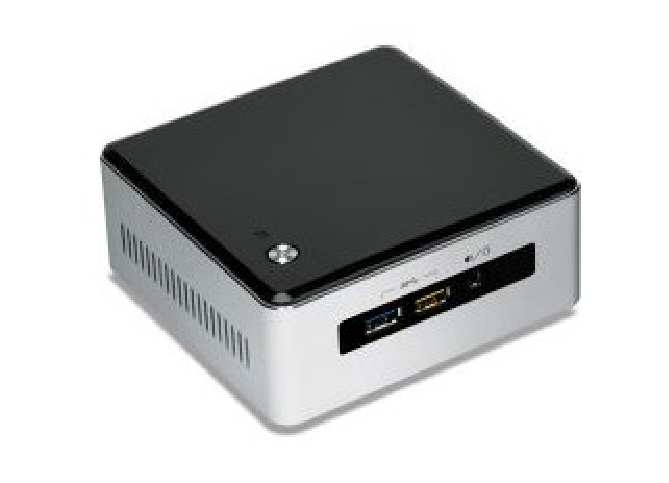
\includegraphics[scale=0.45]{figs/intel-nuc.eps}
\caption{Intel NUC}
\label{NUC}
\end{center}
\end{minipage}
\begin{minipage}{0.5\textwidth}
\begin{center}
\makeatletter
\def\@captype{table}
\makeatother
\caption{Specifications of Intel NUC}
	\begin{tabular}[tbp]{|c|c|}
		\hline 
		External size(WDH) & 115×111×48[mm] \\\hline
		Weight & 0.408[kg] \\\hline
		CPU & Core i5-5250U 1.6[GHz] \\\hline
		Memory & DDR3L 8[GB] \\\hline
	\end{tabular}
\label{table:NUC}
\end{center}
\end{minipage}
\end{figure}

D-UDはメインPCであるNUCと,youBotの内部搭載されたPCと通信しながら,1つのシステムとして動作する.この通信は,車輪の姿勢やオドメトリなどのデータの送受信を頻繁に行うため,LANケーブルを用いた有線接続が必要である.一方,外部からD-UDの操作を行う場合,無線接続したPCから操作することが望ましい.そこで,D-UDのメインPC(NUC)にトラベルルータを接続することで,環境に設置されたWifiに依存することなく,D-UDを無線接続したPCから操作を可能にした(Fig.\ref{computer_connection}).

\begin{figure}[h]
\begin{center}
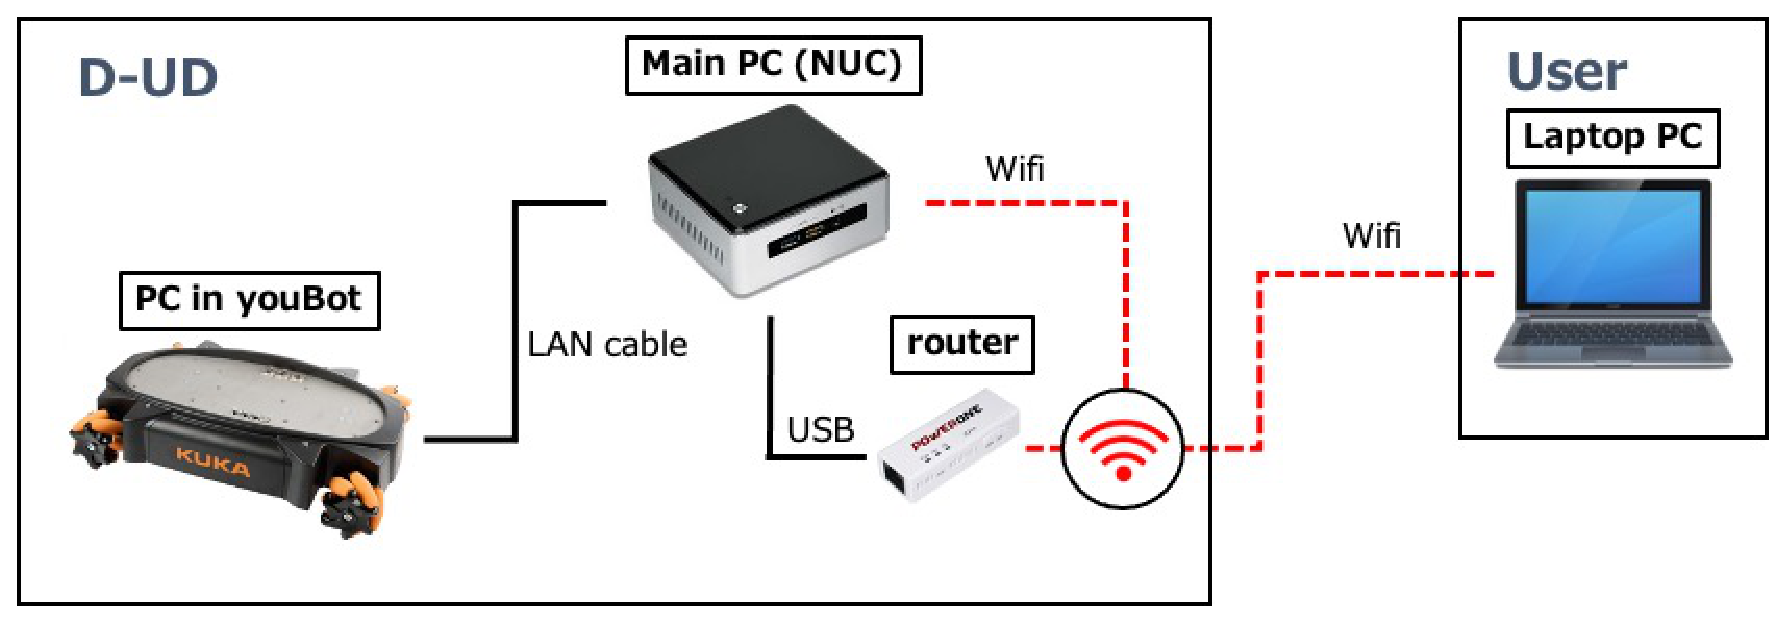
\includegraphics[clip, width=12cm]{figs/configuration.eps}
\caption{Computer connection diagram}
\label{computer_connection}
\end{center}
\end{figure}

\subsection{プロジェクタプラットフォーム}
D-UDのプロジェクタプラットフォームにはFixed-Center Pan-Tilt(FC-PT)機構を採用している(Fig.\ref{pantilt})\cite{pantilt}.プロジェクタで投影した映像の線形的な移動をPan-Tilt機構を用いることで実現する.

\begin{figure}[h]
\begin{center}
\includegraphics[clip, width=6cm]{figs/pantilt.png}
\caption{Picture of Pan-Tilt mechanism}
\label{pantilt}
\end{center}
\end{figure}

\begin{table}[h]
	\caption{Specifications of Pan-Tilt mechanism}
	\label{table:pantilt}
	\centering 
	\begin{tabular}[tbp]{|c|c|}
		\hline 
		External size(WDH) & 220×350×460[mm] \\\hline
		Weight & 5.5[kg] \\\hline
	\end{tabular}
\end{table}

\subsubsection{プロジェクタ}
プロジェクタはLG HF80LSを採用した.Fig.\ref{LG}にLG HF80LSの外観を,Table\ref{table:LG}に仕様を示す.D-UDはプロジェクタを2個搭載する必要があるため,消費電力量の少ないプロジェクタが望ましい.LG HF80LSは,UD2.0で搭載されたプロジェクタ(NEC NP64J)の消費電力が292[w]に対して,140[w]であり約半分の消費電力である.

\begin{figure}
\begin{minipage}{0.4\textwidth}
\begin{center}
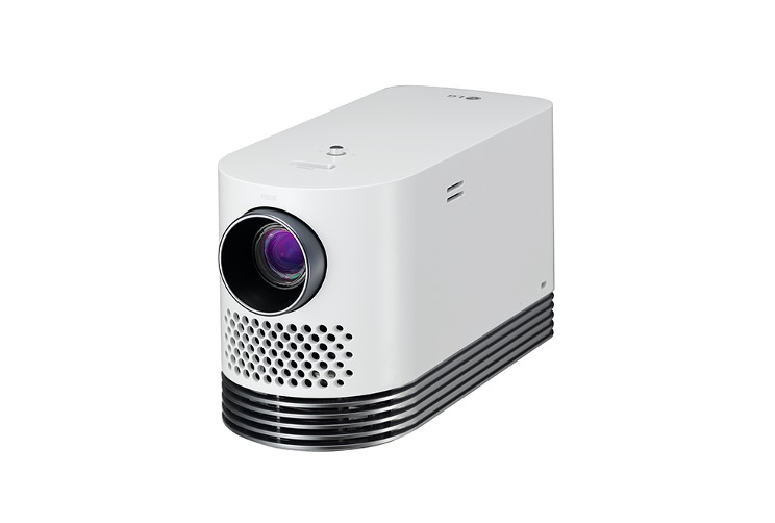
\includegraphics[scale=0.5]{figs/lg_projector.eps}
\caption{LG HF80LS}
\label{LG}
\end{center}
\end{minipage}
\begin{minipage}{0.5\textwidth}
\begin{center}
\makeatletter
\def\@captype{table}
\makeatother
\caption{Specifications of LG HF80LS}
	\begin{tabular}[tbp]{|c|c|}
		\hline 
		External size(WDH) & 108×252×144[mm] \\\hline
		Weight & 2.1[kg] \\\hline
		Resolution & 1920×1080 \\\hline
		Brightness & 2000[lm] \\\hline
		Light source & DLP \\\hline
		Power consumption & 140[w] \\\hline
	\end{tabular}
\label{table:LG}
\end{center}
\end{minipage}
\end{figure}

\subsubsection{パン・チルトモータ}
D-UDではモータとして,Robotis社のDynamixel MX-64ATを使用している.角度制御分解能が高く,円滑な投影画像の移動やぶれの改善が期待できる.MX-64ATの外観をFig.\ref{Dynamixel}に,仕様をTable\ref{table:Dynamixel}に示す.

\begin{figure}
\begin{minipage}{0.4\textwidth}
\begin{center}
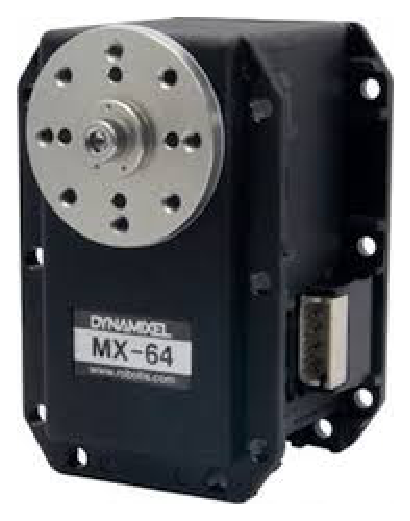
\includegraphics[scale=0.4]{figs/MX_64AT.eps}
\caption{Dynamixel MX-64AT}
\label{Dynamixel}
\end{center}
\end{minipage}
\begin{minipage}{0.5\textwidth}
\begin{center}
\makeatletter
\def\@captype{table}
\makeatother
\caption{Specifications of Dynamixel MX-64AT}
	\begin{tabular}[tbp]{|c|c|}
		\hline 
		Dimensions (WHD) & 40.2x61.1x41[mm] \\\hline
		Weight & 165[g] \\\hline
		Resolution & 4096[pulse/rev] \\\hline
		Stall Torque & 6.0[Nm] \\\hline
		No Load Speed & 63[rev/min] \\\hline
	\end{tabular}
\label{table:Dynamixel}
\end{center}
\end{minipage}
\end{figure}

\subsubsection{プレート}
D-UDは上部のプレートに2台の雲台を搭載させるため,雲台同士の衝突を回避する必要がある.そこで,雲台同士の距離を広げるため,アルミプレートを作成した(Fig.\ref{plate}).

\begin{figure}[t]
\begin{center}
\includegraphics[clip, width=8cm]{figs/top_plate.png}
\caption{Overview of original top plate}
\label{plate}
\end{center}
\end{figure}

\begin{table}[h]
	\caption{Specifications of original top plate}
	\label{table:plate}
	\centering 
	\begin{tabular}[tbp]{|c|c|}
		\hline 
		External size(WDH) & 650×290×5[mm] \\\hline
		Weight & 1.6[kg] \\\hline
	\end{tabular}
\end{table}

\subsection{センサ}
D-UDは異なる位置の人物に向けて情報支援を行う必要がある.

\subsubsection{カメラ}
D-UDに360°パノラマ画像が取得なRICOH Theta Vを搭載した(Fig.\ref{ThetaV}).Theta Vは2枚の魚眼レンズで撮影した円形画像を,正距円筒図法により360°パノラマ画像に変換するカメラである.D-UDは,UD2.1よりも広範囲な環境認識が必要になるためTheta Vを採用している.Theta Vの仕様をTable\ref{table:ThetaV_TABLE}に示す.

\begin{figure}
\begin{minipage}{0.4\textwidth}
\begin{center}
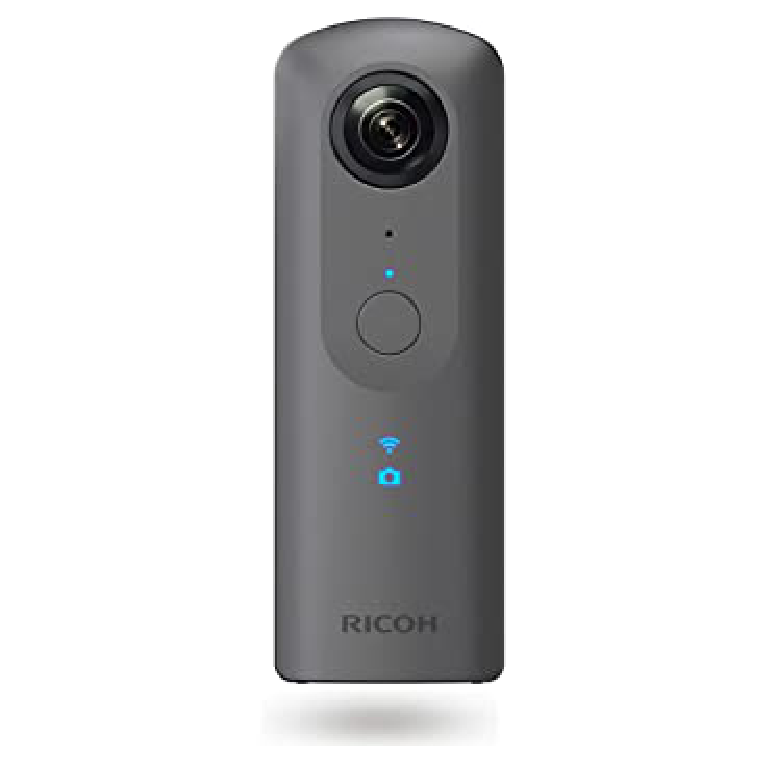
\includegraphics[scale=0.3]{figs/theta_v.eps}
\caption{RICOH Theta V}
\label{ThetaV}
\end{center}
\end{minipage}
\begin{minipage}{0.5\textwidth}
\begin{center}
\makeatletter
\def\@captype{table}
\makeatother
\caption{Specifications of RICOH Theta V}
	\begin{tabular}[tbp]{|c|c|}
		\hline 
		External size(WHD) & 45.2x130.6x22.9[mm] \\\hline
		Weight & 121[g] \\\hline
		Resolution & 1024×512[pixels] \\\hline
		Frame rate & 29.97[FPS] \\\hline
		Connection type & Wifi \\\hline
	\end{tabular}
\label{table:ThetaV_TABLE}
\end{center}
\end{minipage}
\end{figure}

\subsubsection{Laser Range Finder}
D-UDに北陽電機のLaser Range Finder(以後 LRF)であるUTM-30LXを2台搭載している(Fig.\ref{hokuyo}).Fig.\ref{DUD}で示したように,D-UDの前後にLRFを取り付けることで,全方位をセンシングすることができる.このLRFは,D-UDの自己位置推定や障害物等との衝突回避に用いられる.Table\ref{table:hokuyo}にLRFの仕様を示す.

\begin{figure}
\begin{minipage}{0.4\textwidth}
\begin{center}
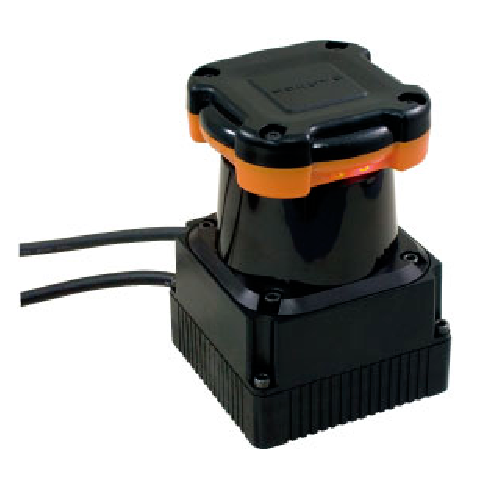
\includegraphics[scale=0.5]{figs/lrf.eps}
\caption{Hokuyo UTM30-LX}
\label{hokuyo}
\end{center}
\end{minipage}
\begin{minipage}{0.5\textwidth}
\begin{center}
\makeatletter
\def\@captype{table}
\makeatother
\caption{Specifications of Hokuyo UTM30-LX}
	\begin{tabular}[tbp]{|c|c|}
		\hline 
		External size(WHD) & 60x60x87[mm] \\\hline
		Weight & 0.37[kg] \\\hline
		Resolution(Distance) & 1.0[mm] \\\hline
		Resolution(Angle) & 0.25[deg] \\\hline
		Accuracy of measure & \begin{tabular}{c}0.1-10[m]:$\pm$ 30[mm]\\10-30[m]:$\pm$50[mm]\end{tabular}\\ \hline
		Scan range(Distance) & 60[m] \\\hline
		Scan range(Angle) & 0.25[deg] \\\hline
		Scanning time(Distance) & 25[msec] \\\hline
	\end{tabular}
\label{table:hokuyo}
\end{center}
\end{minipage}
\end{figure}

%\begin{figure}[h]
%\begin{center}
%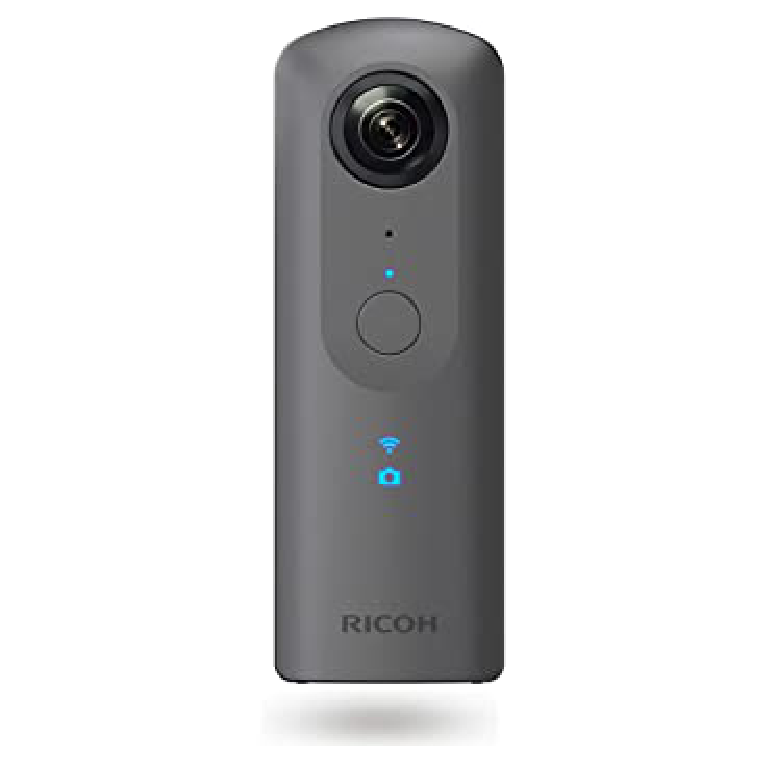
\includegraphics[clip, width=5cm]{figs/theta_v.eps}
%\caption{RICOH Theta V}
%\label{ThetaV}
%\end{center}
%\end{figure}

%\begin{table}[h]
%	\caption{Specifications of RICOH Theta V}
%	\label{table:ThetaV_TABLE}
%	\centering 
%	\begin{tabular}[tbp]{|c|c|}
%		\hline 
%		External size(WHD) & 45.2x130.6x22.9[mm] \\\hline
%		Weight & 121[g] \\\hline
%		Resolution & 1024×512[pixels] \\\hline
%		Frame rate & 29.97[FPS] \\\hline
%		Connection type & Wifi \\\hline
%	\end{tabular}
%\end{table}

\section{ソフトウェア構成}
D-UDの制御には,移動プラットフォームの制御,複数のセンサを使った周囲の環境情報の認識,パン・チルト機構プロジェクタの制御など複数の制御を並列的に処理する必要がある.そこで,本研究ではD-UDの開発において並列処理とコードの再利用性など,ロボット効率的な開発を可能にする,Willow Garage社のROS(Robot Operating System)\cite{ROS}を利用する.

\subsection{ROSミドルウェア}
ROSとは,ロボットソフトウェアプラットフォームの一種である.ROSはノードとよばれるプロセス間で,トピックを介してメッセージを交換することができる.開発者は各プロセスに必要なメッセージの受け渡しを実行することで,容易に各機能の並列処理を行うことができる.D-UDのソフトウェア制御では,各ノードがパブリッシュ・サブスクライブしデータを送受信することで,すべてのプログラムの並列処理を可能にしている.D-UDに実装したコアとなるノード群をFig.\ref{rqt}に示し,各ノードの機能説明をTable\ref{table:ros_node}に示す\footnote{https://github.com/MickeyKen/dual\_ubiquitous\_display\_core}.コアノード群は,アクチュエータやセンサの起動からキーボードやjoystickを用いたD-UDマニュアル操作などのD-UDの基本的な機能を提供する.また,D-UD全体の座標管理やLidarの距離情報を用いたナビゲーション,プロジェクタの投影面の計算も行っている.そのため,開発者は各ノードに必要なデータの通信を考慮するだけで,容易にD-UDのシステムの拡張を行うことができる.

%\ref{chap:control}節にD-UDのコアとなる制御パッケージについて述べる.また,\ref{chap:recognition}節でカメラやLidarを用いた環境認識プログラムの構成について述べる.

\begin{figure}[t]
\begin{center}
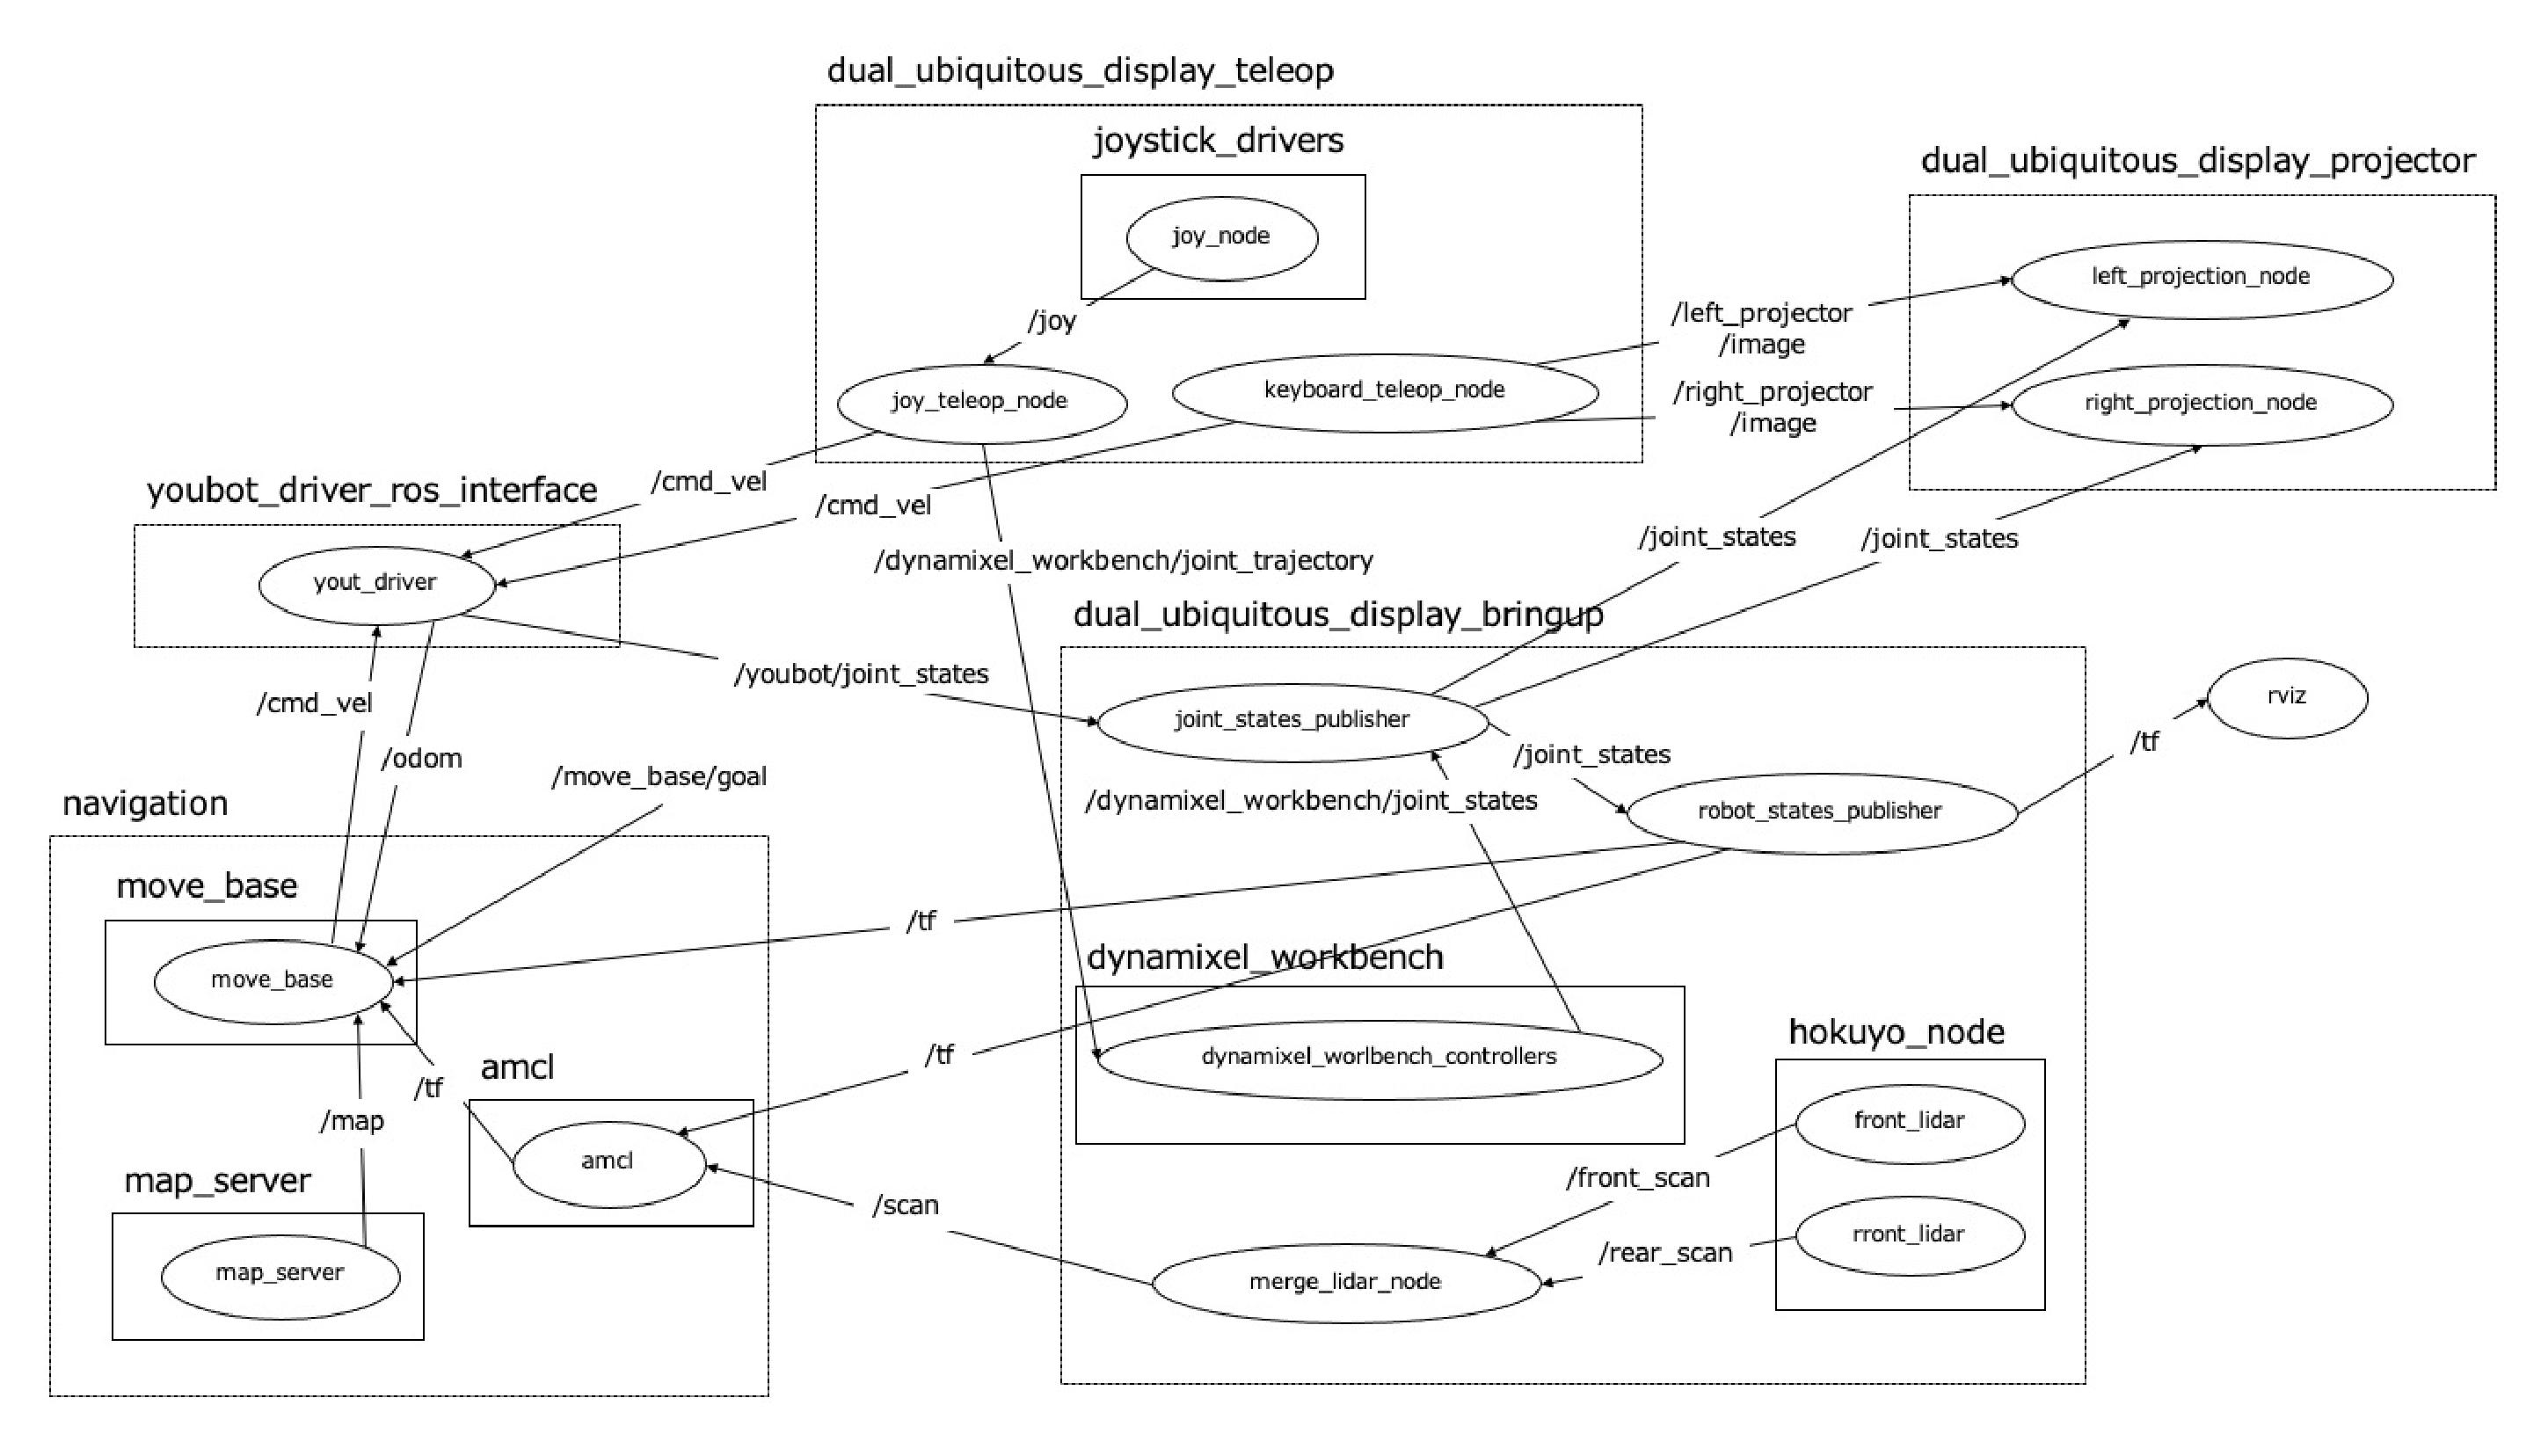
\includegraphics[clip, width=18cm, angle=90]{figs/dud_rqt_graph.eps}
\caption{Nodes and topics}
\label{rqt}
\end{center}
\end{figure}

\begin{table}[t]
\begin{center}
\caption{各ノード名および機能}
\label{table:ros_node}
\scalebox{0.9}[0.9]{
  \begin{tabular}{|c|p{10cm}|}\hline
   ノード名 & 機能説明 \\\hline
   joy\_node & joystickの入力信号を受信して,トピックに変換するノード. \\ \hline
   joy\_teleop\_node & joy\_nodeからパブリッシュされたトピックを受信し,youBotの車輪とパン・チルト機構のモータを制御するトピックをパブリッシュするノード. \\ \hline
   keyboard\_teleop\_node & キーボードの入力信号を受信して,youBotの車輪とパン・チルト機構のモータを制御するトピックをパブリッシュするノード. \\ \hline
   youbot\_driver & 速度のトピックをサブスクライブし,youBotの車輪制御を行うノード. \\ \hline
   move\_base & 目標位置と現在位置のトピックをサブスライブして,経路計画とナビゲーションを実行するノード. \\ \hline
   amcl & Lidarのセンサ値をサブスクライブして,自己位置推定を行うノード. \\ \hline
   map\_server & 事前に作成したマップの画像情報をパブリッシュするノード. \\ \hline
   joint\_states\_publisher & パン・チルト機構のモータやyouBotの車輪の各関節角度を追従し,パブリッシュするノード. \\ \hline
   robot\_states\_publisher & joint\_states\_publisherがパブリッシュするトピックをサブスクライブし,URDFモデルと照合した後ロボットの姿勢のトピックをパブリッシュするノード. \\ \hline
   dynamixel\_workbench\_controllers & パン・チルト機構のモータの目標角度をサブスライブし,Dynamixelを位置制御するノード. \\ \hline
   front\_lidar & D-UDの前方のHokuyo UTM-30LXのセンサ値をパブリッシュするノード. \\ \hline
   rear\_lidar & D-UDの後方のHokuyo UTM-30LXのセンサ値をパブリッシュするノード. \\ \hline
   merge\_lidar\_node & front\_lidarとrear\_lidarからパブリッシュされたトピックをサブスクライブし,それらを統合した後パブリッシュするノード. \\ \hline
   left\_projection\_node & robot\_states\_publisherからパブリッシュされたトピックを受信し,パラメータから取得した画像・動画名を歪み補正して左側のプロジェクタから投影するノード,. \\ \hline
   right\_projector\_node & robot\_states\_publisherからパブリッシュされたトピックを受信し,パラメータから取得した画像・動画名を歪み補正して右側のプロジェクタから投影するノード. \\ \hline

  \end{tabular}
}
  \end{center}
\end{table}

\subsection{ロボットモデリングとシミュレーション}
ROSでは,ロボットの制御の視覚化ツールとシミュレーションツールが存在する.これらのツールを利用することで,ロボットの実機の制御プログラムを開発する際,計算機上でシミュレートすることで,手軽に事前の動作確認が可能となり開発効率が改善される.本研究でも,D-UDの効率的な開発を目指しD-UDのURDF(URDF(Unified
Robot Description)モデルの作成を行った(Fig.\ref{fig:left}).Fig.\ref{fig:right}はRViz(ROS Visualization)という3次元視覚化ツールを用いてD-UDのURDFモデルを表示している.また,シミュレーションツールにはGAZEBO\cite{GAZEBO}が用意されている.GAZEBOは様々なロボットセンサをモデル化するだけでなく,実世界の剛体物理もシミュレーション環境中でモデル化できる3Dロボットモデルシミュレータである.

\begin{figure}[tbp]
	\begin{center}
	\subfigure[Simulation of Dual Ubiquitous Display main body in GAZEBO]{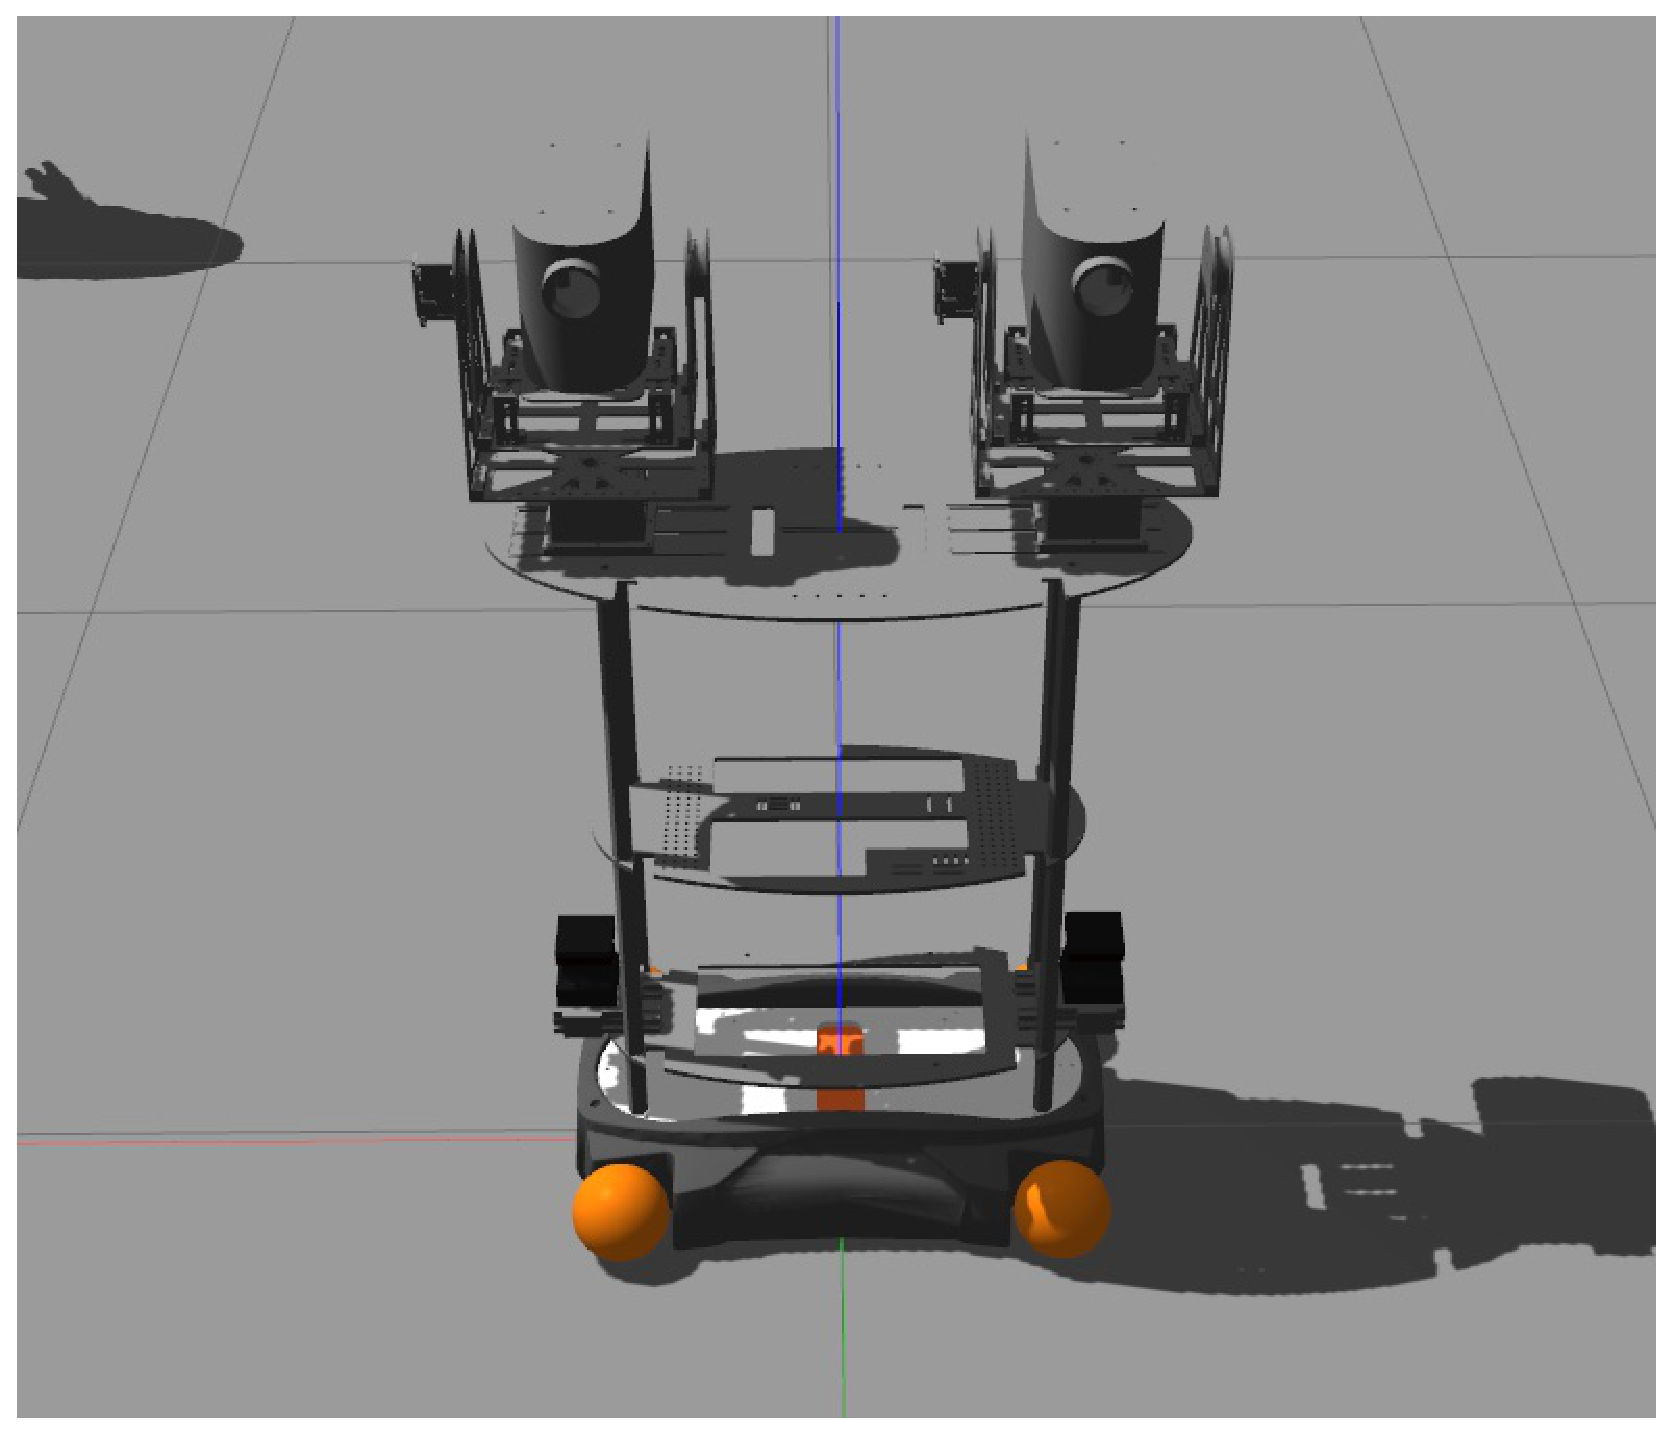
\includegraphics[height=4cm]{figs/dud_gazebo.eps}
	\label{fig:left}}
	\hspace{5mm}
	\subfigure[URDF model of Dual Ubiquitous Display in Rviz]{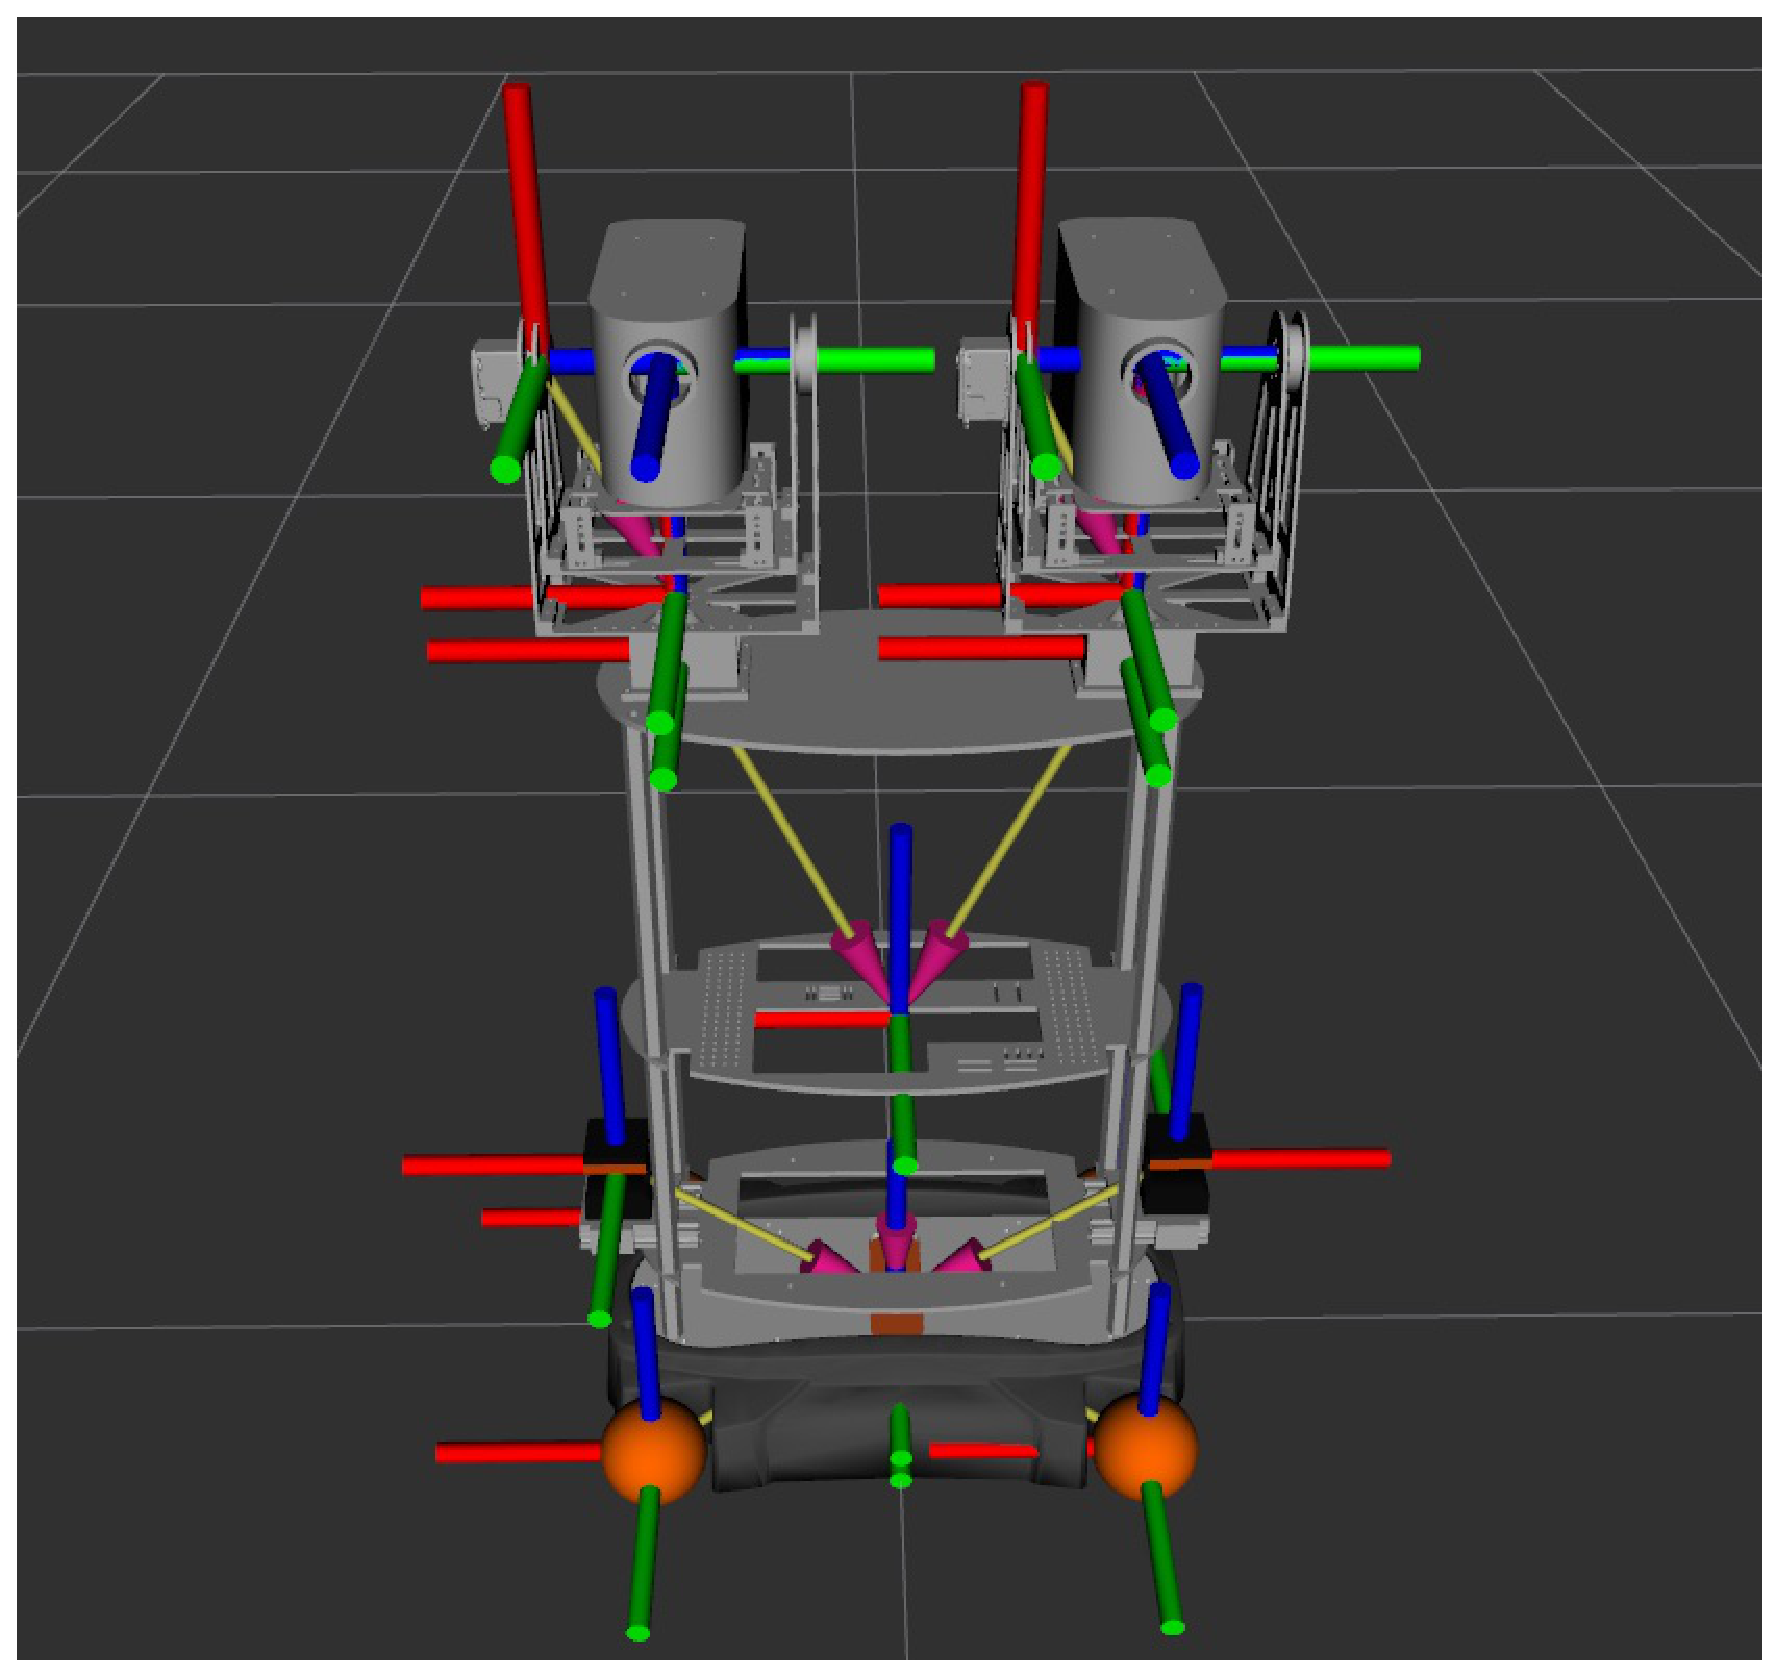
\includegraphics[height=4cm]{figs/dud_urdf.eps}
	\label{fig:right}}
	\subfigure[Dual Ubiquitous Display 3D model in the GAZEBO environment. Blue area indicates the range of LIDAR scanning.]{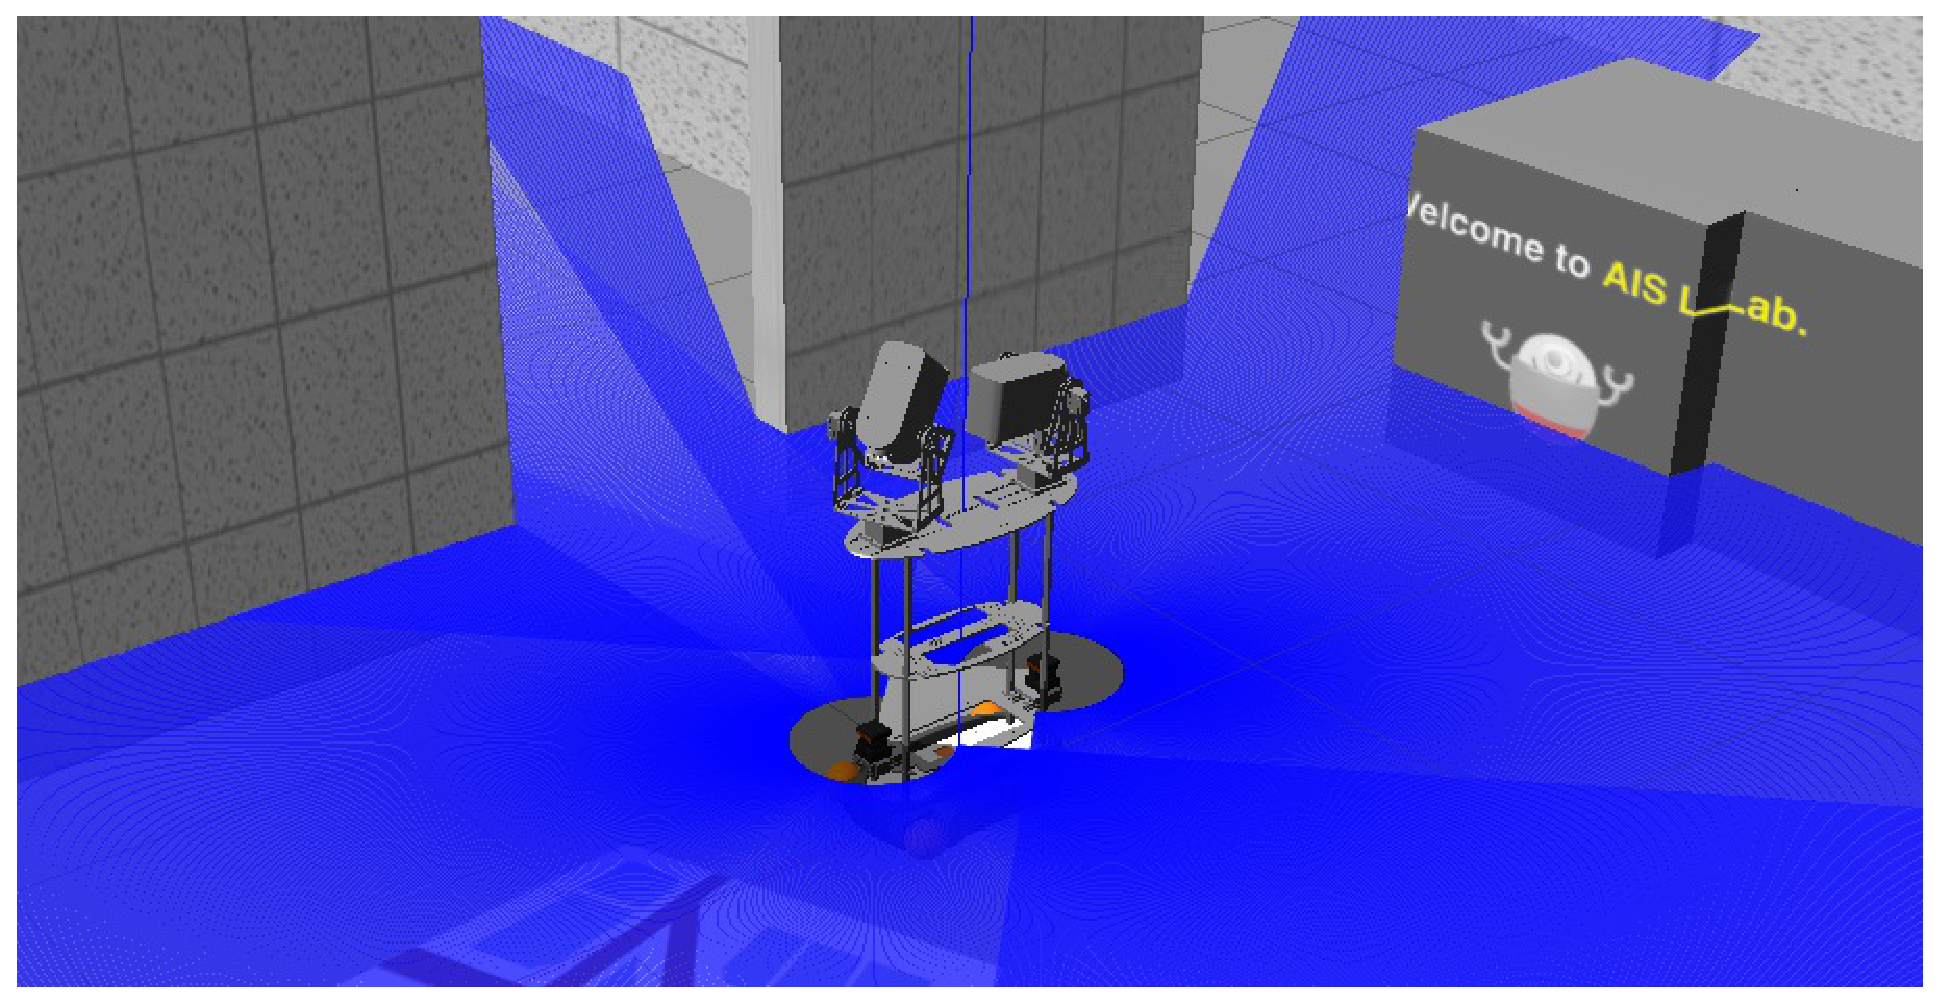
\includegraphics[width=9.2cm]{figs/dud_gazebo_environment2.eps}
	\label{fig:bottom}}
	\end{center}
	\caption{Robot Modeling in GAZEBO/ROS}
	\label{fig:Modeling}
\end{figure}

\chapter{深層強化学習を用いたUDの行動制御}\label{chap:proposal}
第\ref{chap:introduction}章で述べた課題に対する提案手法を詳しく説明する.
章の見出しは「提案手法」とするのではなく,提案内容がわかるように工夫する.

\section{Deep Q-Network(DQN)の概要}
Deep Q-Network (DQN)は,強化学習の手法の一つであるQ学習と,深層ニューラルネットワークを組み合わせて学習させる技術である\cite{drl}. Q学習では,学習主体であるエージェントが状態sで行動aをとったときの行動価値をQ値という値で評価し,ある状態においてQ値が高い行動を選択する方策を学習していく.状態$s_{t}$における行動$a_{t}$のQ値の更新は,以下の式

\begin{equation}
\label{q_update}
Q(s_{t},a_{t} )←Q(s_{t},a_{t} )+ α_{t} (r_{t}+ \gamma maxQ(s_{t+1},a)-Q(s_{t},a_{t}))
\end{equation}

によって更新される.ここで,$r_{t}$はスッテプ$t$での報酬であり,$\gamma$は割引率と呼ばれる$ 0 < \gamma <1 $を満たす定数である.
また,$a_{t}$は学習係数であり,学習の速度を決定する定数である.$maxQ(s_{t+1},a)$は状態$s_{t+1}$における可能な行動の中の最大価値を示している.Q学習はエージェントにQ-tableを用いてQ値の更新を行うが,DQNは学習主体に深層ニューラルネットワークを用いてQ値の更新を行う手法である(Fig.\ref{DQN}).深層ニューラルネットを用いることで,センサ値やロボットの関節角などの状態空間を連続値として入力するが可能となり,学習が収束しやすくなる.

%しかし,エピソードの時系列順で学習を行うと,連続する状態の前後の相関が強いため,学習に偏りが生じる問題がある.そこで,Experience Replayと呼ばれる技術を用いて学習の安定化を図った.Experience Replayは過去の経験${\{s_{t},a_{t},r_{t},s_{t+1}\}}$の系列データをメモリに一度貯めておき,Q関数を推定する際にそれらから無作為に抽出する手法である.

\begin{figure}[t]
\begin{center}
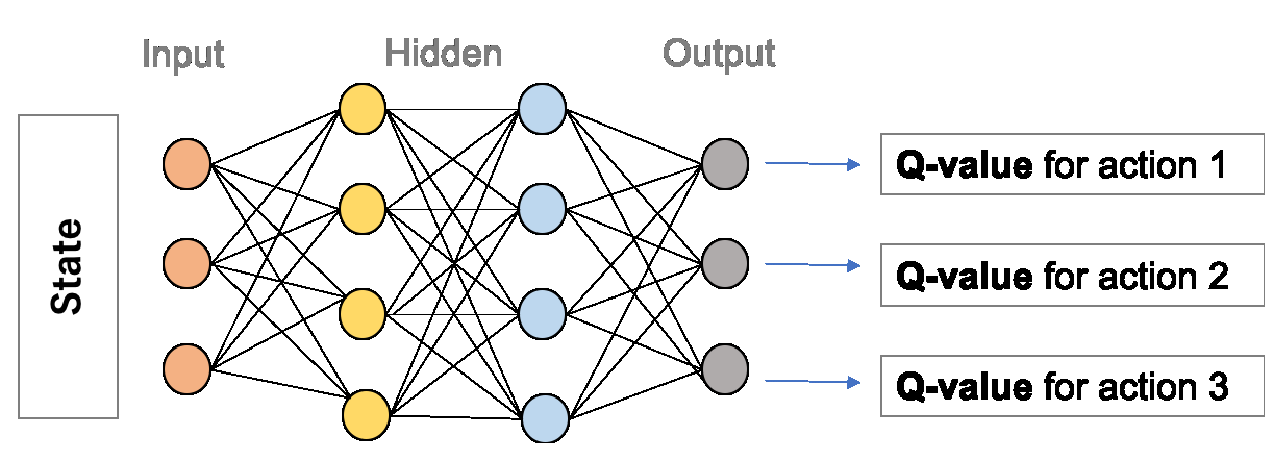
\includegraphics[clip, width=8cm]{figs/dqn_network.eps}
\caption{Deep Q-Network structure}
\label{DQN}
\end{center}
\end{figure}


\section{DQNの効率的な学習手法に関する研究}
深層強化学習を用いた行動最適化は,様々な分野ですぐれた性能を発揮している.しかし,それらの成果物を得るためには,長時間の学習を必要とする.Hasselらは,拡張したDQNを用いてAtariに収録されているゲームをクリアするためには10日の学習日数が必要であると報告している\cite{rainbow}.また,学習時間の問題はロボットの分野でもより深刻な問題となっている.ロボットが環境と相互作用し経験を取得し学習することは,現実世界でもシミュレーション環境においてもゲームよりも複雑な処理をするからである.Zhenらは,物理シミュレーションであるGAZEBO\cite{GAZEBO}の長時間の利用が,処理時間の遅延を引き起こすため,並列処理を用いたロボットの自律移動の学習方法を提案している\cite{pararell}.このように,学習時間を短縮する工夫は,様々な発展を遂げている.よって本章では,学習時間の短縮を目指した学習の安定化・効率化および分散学習の技術について述べる.

\subsection{Double Deep Q-Network (DDQN)}
DQNは,最適な行動$a$を選択するネットワークと行動価値を評価するネットワークを同一のモデルで学習を行う.つまり,式(\ref{q_update})で示したとおり,次の状態の最大のQ値を求めるときに自身のネットワークを用いて計算している.しかし,ネットワークのパラメータ更新時に$Q(s,a)$の上方向の誤差が生じるため,行動$a$を過大評価してしまう恐れがある.そこで,Hasseltらは行動選択のネットワークと評価するネットワークを分けて学習を行うDDQNを提案している\cite{double}.パラメータ更新に必要なTD誤差の計算において,$maxQ(s_{t+1},a)$の計算を行うネットワークを$Q_{main}$とし,その行動の評価を行うネットワークを$Q_{target}$とするとQ値の更新式は以下のように書ける.

\begin{equation}
\label{a_main}
a_{main}=argmaxQ_{main}(s_{t+1},a)
\end{equation}

\begin{equation}
\label{double_q_update}
Q(s_{t},a_{t} )←Q(s_{t},a_{t} )+ α_{t} (r_{t}+ \gamma maxQ_{target}(s_{t+1},a_{main})-Q(s_{t},a_{t}))
\end{equation}

\subsection{Multi-step Learning}
Multi-step Learningは行動修正を行う際,複数ステップを考慮する手法である\cite{rl_book}.強化学習において,行動の修正の方法は,実績から修正を行うMonte Carlo法と予測して修正を行うTD法(Temporal Difference Learning)の2つに分かれる.前者のMonte Carlo法の特徴として,実際に獲得した即時報酬の総和から行動を修正するため,正確な行動修正が可能であるが,エピソードが終了するまで修正することができない問題点がある.一方,TD法はエピソード終了までの合計報酬を予測して,行動を修正するためエピソードの途中でも行動修正が可能であるが,予測に基づくため正確性に欠ける問題がある.Multi-step Learning法はこれらの手法の中間に位置する手法である.よって,合計報酬の式は即時報酬と予測を合わせた以下のように定義される.

\begin{equation}
\label{multi-step}
G_{t}=R_{t+1}+\gamma R_{t+2}+\cdots+\gamma^{n-1}R_{t+n}+\gamma^n Q(s_{t+1},argmaxQ(s_{t+n},a))
\end{equation}

ここで,$\gamma(0<\gamma<1)$は割引率であり即時報酬獲得の不確かさを表す係数である.
\subsection{Prioritized Experience Replay}
Prioritized Experience Replay(PER)は,TD誤差の大きい経験から優先してサンプリングを行う手法である\cite{prioritized}.TD誤差の大きい経験は,高報酬を得たものや,非常に悪い行動を選択したものなど学習効率が高いものが多く,効率的に学習を進めることができる.ここで,TD誤差$\delta_{j}$を以下のように定義する.
\begin{equation}
\label{TD_error}
  \delta_{j}=r(s_{t},a_{t})+\gamma Q^{\prime}(s_{t+1},a_{t+1},w)-Q(s_{t},a_{t},w)
\end{equation}

しかし,TD誤差による優先度では,最初にTD誤差が小さくなった経験は,リプレイされずに長時間放置されるといった問題がある.また,TD誤差が大きいものばかり優先されることで,経験の多様性が失われ過学習につながるおそれがある.そこで,確率的サンプリング手法を用いて確率的に選択する手法が提案されている.
\begin{equation}
\label{sum_P_i}
  P(i)=\frac{D_{i}^{\alpha}}{\sum_{k}D_{k}^{\alpha}}
\end{equation}

ここで,$D_{i}=\frac{1}{rank(i)}>0$と定義され,$rank(i)$はリプレイブッファ内の経験$i$の絶対値の大きさの順位である.また,PERはprioprityに基づく確率により,replayに使うデータをサンプリングすることによりデータの分布を変えてしまうため,推定している期待値のバイアスが大きくなる.そこで,このバイアスを是正するために,サンプリングされる確率の大きいデータほど,lossへの寄与を小さくし,重要度重み(Important Sampling(IS) Weights)を経験に掛けてデータに補正をかける.

\subsection{深層強化学習の分散アーキテクチャ}
エージェントを分散させて,学習する仕組みが近年盛んに研究されている\cite{A3C}\cite{Gorila}\cite{Ape-X}.Mnihらは分散環境を使用した方策勾配法による深層強化学習の手法を提案している\cite{A3C}.A3C(Asynchronous Advantage actor-critic)のエージェントは,各環境でデータ収集だけでなく学習も行う.しかし

\section{提案手法の概要}
\subsection{UDが情報支援を行うための前提条件}
\subsection{GAZEBOとROSを用いた分散アーキテクチャ}
\subsection{DQNを用いた行動制御}

\chapter{実験}
\section{シミュレーションを用いた実験}
\section{実験方法}
\section{実験結果}
\section{考察}
\section{実機を用いた実験}
\section{実験方法}
\section{LidarとRGBカメラを用いた人物の位置・向き検出}
実機実験において,目標人物の検出を2D Lidarと魚眼カメラを用いて行った.魚顔カメラは180度のRGB情報が取得可能なELP社のELP-USB8MP02G-L180を採用した.本システムはRGB画像情報から目標人物の検出を行った後,検出した目標人物の矩形内にあるLidarの値を用いて,脚と顔の向きから目標人物の立ち位置と向きを推定する.本システムの2D Lidarによる脚検出には,ROS公式のpeopleスタック\footnote{https://github.com/wg-perception/people}の一部であるleg\_detectorノードを用いた.また,RGB画像による人物の検出には,深層学習をアルゴリズムに持ち様々な物体を検出可能なIntel OpenVinoパッケージ\footnote{https://github.com/intel/ros\_openvino\_toolkit}を利用した.

\begin{figure}[t]
\begin{center}
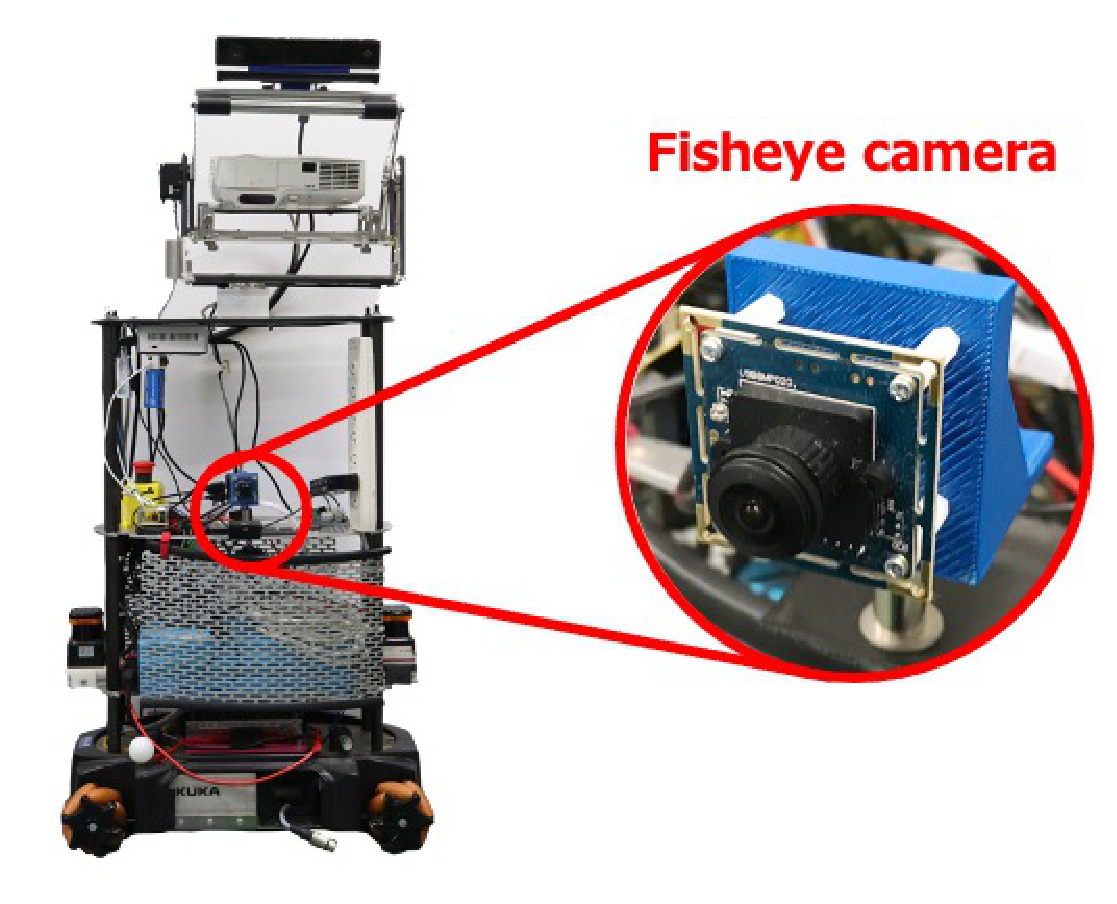
\includegraphics[clip, width=8cm]{figs/ud_with_fisheyecamera.eps}
\caption{Overview of fisheye camera}
\label{ud_with_fisheyecamera}
\end{center}
\end{figure}

\section{実験結果}
\section{考察}

\chapter{結言}
最後に結論をまとめる.
原則として,新たな内容は書かずに今まで書いたことを再度まとめて書く.

また,今後の課題(やり残していること)についても最後に触れる.

\chapter*{謝辞}
謝辞を書く.謝辞には章番号はつかない.


%参考文献
% BibTeXを使用する.
% ※platexを実行(ビルド)した後にpbibtexを実行し,再度platexを実行(ビルド)しないと反映されない
% BibTexを使用しない場合は,以下の2行のコメントアウトする 
\bibliographystyle{sonota/aislab.bst} % 文献の参照スタイルの指定(aislab.bstを見に行く)
\bibliography{aislab.bib} % 文献データベース(bibファイル)の指定

%参考文献 BibTexを使用しない場合は,以下の\begin{comment}と\end{comment}の行を削除する
\begin{comment}
\begin{thebibliography}{1}
\bibitem{test1}
 athor1,  author2,  author3, ``title1'',  booktitle1, pp. 2--181--2--182, 2009.
\bibitem{test2}
 athor1,  author2, ``title2'',  booktitle2, pp. 137--142, 2010.
\bibitem{test3}
 athor1, ``title3'',  booktitle3, pp. 134--143, 2013.
\end{thebibliography}
\end{comment}

\end{document}
